\documentclass[fontsize=8pt, a4paper, fleqn, landscape, DIV=calc]{scrartcl}
\usepackage[utf8]{inputenc}
\usepackage[ngerman]{babel}

\usepackage{hyperref}%links in the pdf
\hypersetup{pdfborder = {0 0 0}}%No borders around Hyperlinks

%Layout
\usepackage{multicol, geometry, tcolorbox, fancyhdr, lastpage, dirtytalk, qrcode, rotating}
% mehrere spalten, page layout, farbboxen der titel, header/footer, linkt to last page, make the use of "" easier, QR code im Titel, Rotate tables
\geometry{margin=1cm}
\parindent 0pt
\pagestyle{fancy}
\newlength{\breite}
\setlength{\breite}{0.5pt}
\setlength{\columnseprule}{\breite}

\usepackage[table,xcdraw]{xcolor}% color

%Math stuff
\usepackage{mathtools}
%\allowdisplaybreaks %allow display breaks in align

%\newcommand{\todo}[1][todo]{% Todo marker
%    \begin{tcolorbox}[colback=orange, beforeafter skip=2pt, boxrule=0pt, arc=2pt, left=0pt, right=0pt, top=0pt, bottom=0pt]%
%        {#1}%
%    \end{tcolorbox}%
%} 
% Todo no longer alowed


%automate Columnbreak
\newcommand{\nextcol}{%
\vfill\null%
\columnbreak%
}

\usepackage{enumitem}%Itemise 

%Display Code
\usepackage{listings}
\definecolor{codeGreen}{RGB}{69, 161, 18}
\definecolor{backgroundcolor}{RGB}{255,255,255}
\lstdefinestyle{mystyle}{
    language = [11]C++,
    backgroundcolor=\color{backgroundcolor},
    commentstyle=\color{blue},
    keywordstyle=\color{codeGreen},
    numberstyle=\tiny\color{black},
    stringstyle=\color{olive},
    basicstyle=\ttfamily\footnotesize,
    breakatwhitespace=false,         
    breaklines=true,                  
    captionpos=b,                    
    keepspaces=true,                 
    numbers=none,                    
    numbersep=5pt,                  
    showspaces=false,                
    showstringspaces=false,
    showtabs=false,                  
    tabsize=2,
    morekeywords  = {[11]final, override}
}
\lstset{style=mystyle}

\usepackage{ifthen} % ifthen to let others use this document, based on their setup
\newboolean{tikzumlWorks}
\setboolean{tikzumlWorks}{true} % false = tikzumlpackage NOT installed

\newboolean{svgWorks}
\setboolean{svgWorks}{true} % false = svg package NOT installed

\ifthenelse{\boolean{tikzumlWorks}}{
    \usepackage{tikz-uml} % for this to work, download tikz-uml.sty from https://perso.ensta-paris.fr/~kielbasi/tikzuml/index.php?lang=en to 'texlive/texmf-local/tex/latex/local' and run 'texhash' in ps terminal (windows)
    \tikzumlset{fill class=subsectionbarcolor!50}
    }{}

\ifthenelse{\boolean{svgWorks}}{
    \usepackage{svg}
    \svgpath{{svg/}}
    }{}


% color for  Titel / sub Titel
\definecolor{sectionbarcolor}{RGB}{148,0,255}
\definecolor{subsectionbarcolor}{RGB}{220,173,255}
\definecolor{sectiontextcolor}{RGB}{255,255,255}
\definecolor{subsectiontextcolor}{RGB}{0,0,0}

%section color box
\setkomafont{section}{\mysection}
\newcommand{\mysection}[1]{%
    \Large%
    \begin{tcolorbox}[colback=sectionbarcolor, coltext=sectiontextcolor, beforeafter skip=1pt, boxrule=0pt, arc=2pt, left=0pt, right=0pt, top=0pt, bottom=0pt]%
        {#1}%
    \end{tcolorbox}%
}

%subsection color box
\setkomafont{subsection}{\mysubsection}
\newcommand{\mysubsection}[1]{%
    \Large%
    \begin{tcolorbox}[colback=subsectionbarcolor, coltext=subsectiontextcolor, beforeafter skip=1pt, boxrule=0pt, arc=2pt, left=0pt, right=0pt, top=0pt, bottom=0pt]%
        {#1}%
    \end{tcolorbox}%
}

%Information for maketitle
\title{\vspace{-1cm}Prog C++}
\subtitle{FS 2024, Prof. Dr. Christian Werner}
\author{Fabian Steiner, \today}
\date{{\small 1.1.7}}

%Header & footer
\fancyhf{}
\setlength{\footskip}{0.5cm}
\fancyfoot[L]{\thepage{} / \pageref{LastPage}}
\fancyfoot[R]{C++}
\renewcommand{\footrulewidth}{0pt}
\renewcommand{\headrulewidth}{0pt}

\begin{document}
	\begin{multicols*}{3}
        \raggedcolumns
        \begin{minipage}[c]{0.75\columnwidth}
		      \maketitle
        \end{minipage}
        \begin{minipage}[c]{0.2\columnwidth}
            \begin{center}
                \quad
                \qrcode[height=\linewidth]{https://github.com/Iceteavanill/Cheatsheet-Prog_Cpp_FS_2024_OST}
                \qquad    
            \end{center}
        \end{minipage}
        
        \thispagestyle{fancy}%Pagenumber for first page

        \section{Basics}

\subsection{Trivia}

Entstanden durch Stroustrup 1986.\\

\subsection{Grundsätzlich}

C++ ist sehr ähnlich zu C. Es gibt aber einige Wichtige Änderungen zu C:

\begin{itemize}[itemsep=1pt, parsep=0pt]
    \item zu benutzender Compiler heisst jetzt \say{clang++}
    \item Nativen Bool Typ : \textbf{Bool}
    \item richtiges Konstanten Schlüsselwort : \textbf{constexpr}
    \item Standartbibliotheken haben kein .h mehr beim Aufrufen
    \item Char-Literale (z. B. 'A') haben in C++ den Datentyp char (in C war es int)
    \item Es gibt benannte Namensräume. Wichtigster Namensraum für die STL: std
    \item ...
\end{itemize}

\subsection{Sourcecode Hello world CPP}

\lstinputlisting[language = c++]{code/hello_World.cpp}

\subsection{Streams}

Ein Stream repräsentiert einen generischen sequentiellen Datenstrom. Z.b: ein Enigabefeld, Dateien oder Netzwerktraffic.\\
Die wichtigsten Operatoren sind:

\begin{itemize}[itemsep=1pt, parsep=0pt]
    \item \textbf{$<<$} Inserter $\rightarrow$  Daten einfügen
    \item \textbf{$>>$} Extractor $\rightarrow$ Daten herausholen
\end{itemize}

Für definierte Klassen sind diese Operatoren bereits definiert.

\subsubsection{Standardstreams}

\begin{itemize}[itemsep=1pt, parsep=0pt]
    \item \textbf{cin} Standart Eingabe
    \item \textbf{cout} Standart Ausgabe
    \item \textbf{cerr} Standart Fehlerausgabe
    \item \textbf{clog} Mit cerr gekoppelt aber etwas anders
\end{itemize}

\subsubsection{Streamformatierung}

Formatierungen der Streams kann mit folgenden Schüsselwörtern erreicht werden:


\begin{center}
    \begin{tabular}{cc}
        \rowcolor[HTML]{EFEFEF} 
        \textbf{Flag} & \textbf{Wirkung}                                        \\ \hline
        boolalpha     & bool-Werte werden textuell ausgegeben                   \\
        dec           & Ausgabe erfolgt dezimal                                 \\
        fixed         & Gleitkommazahlen im Fixpunktformat                      \\
        hex           & Ausgabe erfolgt hexadezimal                             \\
        internal      & Ausgabe innerhalb Feld                                  \\
        left          & linksbündig                                             \\
        oct           & Ausgabe erfolgt oktal                                   \\
        right         & rechtsbündig                                            \\
        scientific    & Gleitkommazahl wissenschaftlich                         \\
        showbase      & Zahlenbasis wird gezeigt                                \\
        showpoint     & Dezimalpunkt wird immer ausgegeben                      \\
        showpos       & Vorzeichen bei positiven Zahlen anzeigen                \\
        skipws        & Führende Whitespaces nicht anzeigen                     \\
        unitbuf       & Leert Buffer des Outputstreams nach Schreiben           \\
        uppercase     & Alle Kleinbuchstaben in Grossbuchstaben wandel         
    \end{tabular}
\end{center}




        \section{Objektorientierung}

Objektorientierung soll es erleichtern eine Abbildung der Realität zu erstellen. 
Viele Dinge aus der Wirklichkeit können als Modell dargestellt / simplifiziert werden. 
Diese Modelle können in Software in sogenannte Objekte \say{umgewandelt} werden.

\subsection{Objekte}

Objekte stellen Dinge, Sachverhalte oder Prozesse dar. Sie sind ein rein gedankliches Konzept.\\
Sie kennzeichnen sich durch:

\begin{itemize}[itemsep=1pt, parsep=0pt]
    \item eine \textbf{Identität}, welche es erlaubt Objekte voneinander zu unterscheiden
    \item \textbf{statische Eigenschaften} zur Darstellung des \textbf{Zustandes} des Objekts in Form von \textbf{Attributen}
    \item \textbf{dynamische Eigenschaften} zur Darstellung des \textbf{Verhaltens} des Objekts in Form von \textbf{Methoden}
\end{itemize}


\subsection{Klassen \& Instanzen}

Ähnliche Objekte können in \textbf{Klassen} zusammengefasst werden, um Programmieraufwand tiefer zu halten. 
Verwendete Objekte werden als \textbf{Instanz} eingesetzt. Diese Objekte haben dieselben Attribute, allerdings andere Werte.\\
Eine Beispielklasse:\\

\lstinputlisting{code/class_example.cpp}

\nextcol

\subsubsection{Header-Datei}

Reihenfolge in der Header-Datei:

\begin{enumerate}[itemsep=1pt, parsep=0pt]
    \item Dateikommentar mit Lizenzvereinbarung.
    \item \textit{\color{blue} \say{Includes} des verwendete System Header}
    \item \textit{\color{blue} \say{Includes} der Projektbezogenen Header}
    \item \textit{\color{blue} Definition von Konstanten}
    \item \textit{\color{blue} Typedef's und Definitionen von Strukturen}
    \item \textit{\color{blue} allenfalls extern-Deklaration von Global-Variablen}
    \item \textit{\color{blue} Funktionsprototypen, ink. Kommentar der Schnittstelle, bzw. Klassendeklarationen}
\end{enumerate}

Die \textit{blauen} Punkte müssen sich im Includeguard befinden(\#pragma once). 
Pro Header-Datei sollte nur eine Oberklasse deklariert sein. 
Kleine Unterklassen können im gleichen Header stehen.

\subsubsection{Reihenfolge der Implementation}

\begin{enumerate}[itemsep=1pt, parsep=0pt]
    \item Dateikommentar mit Lizenzvereinbarung
    \item \say{includes} der eigenen Header
    \item \say{includes} der Projektbezogenen Header
    \item \say{includes} der verwendeten System Header
    \item allenfalls globale und statische Variablen
    \item Präprozessor-Direktiven
    \item Funktionsprototypen von lokalen, internen Funktionen (in nameless Namespace)
    \item Definition von Funktionen und Klassen
\end{enumerate}

\subsection{UML}

Die \say{Unified Modeling Language} ist eine normierte Sprache um Objekte grafisch darzustellen. 
Sie geht extrem ins Detail. 
Darum hier nur ein Ausschnitt:

\subsubsection{UML-Klassendiagramm Notation}

Besteht immer aus 3 Boxen:\\

\noindent
\begin{minipage}{0.6\columnwidth}
\begin{center}
    \ifthenelse{\boolean{tikzumlWorks}}{
    \begin{tikzpicture} 
        \umlclass{Student}{ 
            + IDNumber : int \\ \#{} name : std::string \\ - bierkonsum : float \\ \# investedTimeInET : long int 
            }{ 
            - doStuff(time : int\&) : void \\ + \textit{useless(void) : (retType)*}
        }
    \end{tikzpicture}  
    }{
        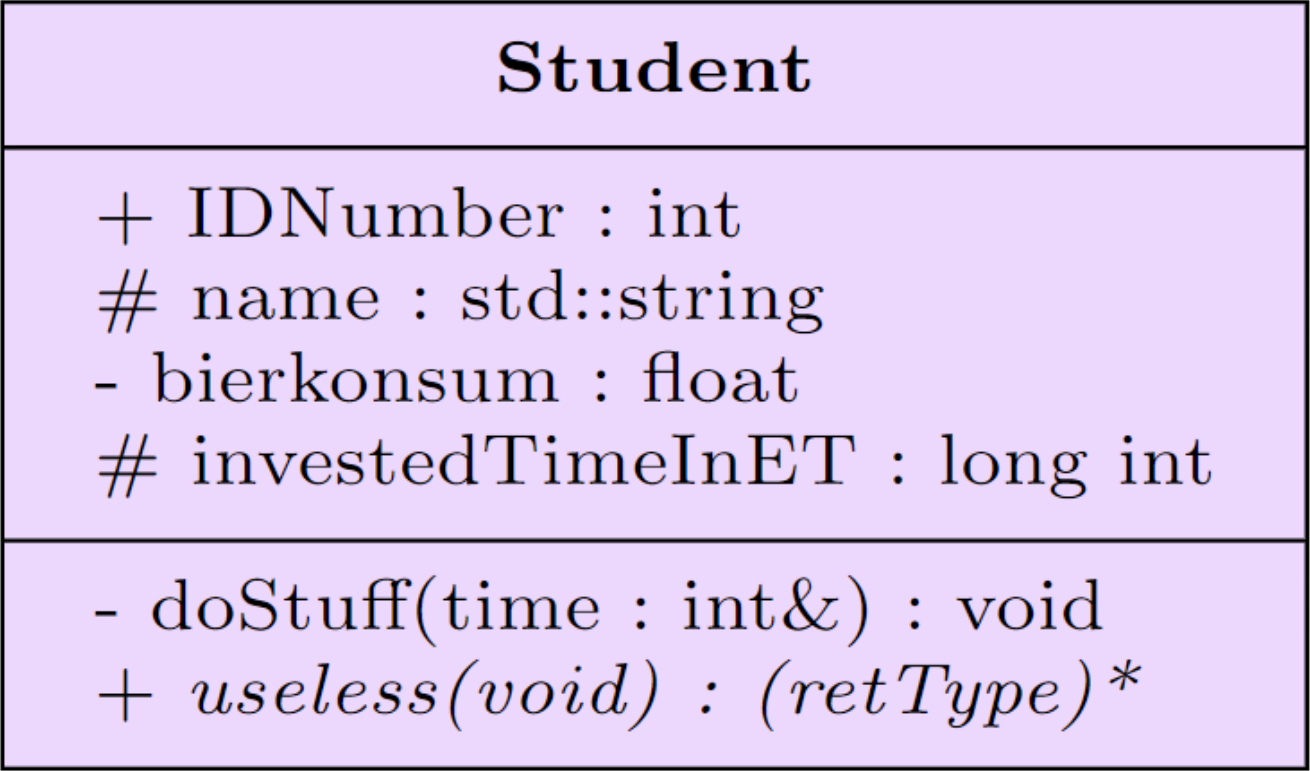
\includegraphics[width=0.8\columnwidth]{pictures/UML-Klassendiagramm Notation.png}    
    }
\end{center}
\end{minipage}
\begin{minipage}{0.4\columnwidth}

    Zu oberst der Name, in der Mitte Attribute(Variablen) und unten Methoden.
    Die Methoden und Attribute fangen mit einem Symbol, an welches die Sichtbarkeit definiert und haben ein bestimmtes Merkmal:

\end{minipage}

\begin{itemize}[itemsep=1pt, parsep=0pt]
    \item + : public (überall sichtbar)
    \item - : private (nur in  aktueller Klasse sichtbar)
    \item \# : protected (in aktueller und Unterklassen sichtbar)
    \item \textit{Italic} :  Funktion oder Klasse ist Abstrakt (=0)
    \item \underline{Unterschrichen} : Funktion oder Attribut ist static
    \item $<\text{Name der Klasse}>$ :  Konstruktor
    \item $\sim<\text{Name der Klasse}>$ : Destruktor
\end{itemize}



\subsubsection{class \& struct im Zusammenhang mit Objekten}

Eine class und struct können fast identisch verwendet werden. 
Eine class hat standardmässig Sichtbarkeit private, Struct public(wenn nichts definiert wird).

\subsection{Inkludierte Dokumentation}

Mann kann im H-File direkt die Dokumentation zu der Schnittstelle schreiben. 
Das ermöglicht das einfachere Verwenden der Schnittstelle.
Dies wird in einem Blockkommentar, nach folgendem Muster realisiert:

\lstinputlisting{code/codedocumentation.cpp}

Es kann immer mehr geschrieben werden, man sollte sich aber auf das Nötige beschränken.

\section{Konstruktoren und Destruktoren}

Konstruktoren und Destruktoren sind spezielle Methoden von Klassen. 
Diese haben immer denselben Namen wie die Klasse und \textbf{kein} Rückgabetyp(auch nicht void).\\
Aufrufparameter haben folgende Bedeutung:

\begin{itemize}[itemsep=1pt, parsep=0pt]
    \item \textbf{\say{Keine}} : Default Konstruktor
    \item \textbf{\say{const-Referenz auf eigene Klasse}} : copy Konstruktor
    \item \textbf{Alles andere} : User-Defined
\end{itemize}

\subsection{Konstruktoren}

Konstruktoren bereiten die Instanz auf ihre Funktion vor. \\

Wichtig ist, dass ein Konstruktor immer \textbf{alle} Attribute der Klasse initialisiert.
Konstruktoren werden wie folgt aufgerufen:\\

\subsubsection{User-Defined}

\begin{itemize}[itemsep=1pt, parsep=0pt]
    \item Default $\rightarrow$ ohne Aufrufparameter
    \item Copy $\rightarrow$ mit einer const Referenz auf eine andere Instanz
    \item sonstige $\rightarrow$ werden anhand ihrer Aufrufparameter unterschieden, Sprechweise:\say{überladen}
\end{itemize}

Werden verschiedene Konstruktoren definiert, muss der Default zuerst aufgerufen werden, wenn dieser erhalten bleiben soll.\\

\subsubsection{Implizit}

Falls ein expliziter nicht angegeben wurde, dieser jedoch aus technischen Gründen benötigt wird:

\begin{itemize}[itemsep=1pt, parsep=0pt]
    \item Default $\rightarrow$ macht nichts, alle Parameter bleiben uninitialisiert
    \item Copy $\rightarrow$ dieser kopiert alle Attribute der anderen Instanz eins-zu-eins(bytewise). Problematisch, wenn die Instanz Pointer auf etwas hat.
    \item ...
\end{itemize}

Wenn ein Objekt einen Pointer auf einen allokierten Speicher hat, muss eine spezielle Copy Methode verwendet werden. 
Der Pointerwert / Adresse wo dieser hinzeigt, wird einfach kopiert. 
Falls dann das erste Objekt den Speicher freigibt, wird die Speicheralokation gelöscht. 
Sobald Objekt 2 nun den Speicher aufruft, zeigt dieser auf ungültigen Speicher $\rightarrow$ \textit{Segmentation fault}.\\
Darum \textbf{MUSS} dem Objekt ein separater Speicherbereich gegeben werden.\\

Merke: Konstruktoren werden immer dann gerufen (evtl. auch \textbf{implizit}) wenn ein neues Objekt in den Speicher gelegt wird.\\

\subsection{Destruktor}

Destruktoren entfernen das Objekt aus dem Speicher. 
Hat keine Aufrufparameter und auch kein Rückgabewert. 
Es kann immer nur \textbf{einen} Destruktor geben
Wenn der Destruktor fertig ist, sollte kein Speicher mehr vom Objekt belegt sein.\\
Destruktoren sollten immer \textbf{Virtuell definiert werden} (siehe \ref{Virtual}). 
Mit anderen Virtuellen Funktionen \textbf{müssen} sie Virtuel definiert werden. 
Der Funktionsname beginnt mit einer Tilde. 
Der Destruktor wird evtl. auch Implizit aufgerufen z.b., wenn aus einer Funktion wieder herausgesprungen wird. 

\subsection{Beispiel}

\lstinputlisting{code/constructor.cpp}

\section{Initialisierungslisten und direkte Initialisierung}

Die Initialisierung von Datentypen kann auf verschiedene Arten erreicht werden. 
Es wird zwischen Zuweisung und Initialisierung unterschieden.

\subsection{POD's}

\say{plain old datastructure} / built in datatypes

\lstinputlisting{code/pod_init.cpp}

\subsection{Non PODs}

\lstinputlisting{code/non_pod_init.cpp}

\nextcol

\subsection{User defined Constructor}

Um eine Klasse richtig initialisieren zu können muss der Ctor korrekt definiert werden. 
Eine sogenannte Initialisierungsliste wird verwendet:

\lstinputlisting{code/userdefined_ctro.cpp}

\section{Assertions}

Assertions sollten Annahmen über korrekte Wertebelegung darstellen. 
Sie sind kein C spezifisches Konzept und sollten \textbf{nur zu Testzwecken} eingesetzt werden. 
Im Releasebuild sollten sie deaktiviert werden. 
Dafür gibt es spezifische Präprozessorflags.
Der Header \textbf{$<$assert.h$>$} bzw. \textbf{$<$cassert$>$} stellt hierfür ein Präprozessor-Makro \say{assert(Bedingung)} zur Verfügung, um solche Zusicherungen auszudrücken.\\
Beispiel:\\

\lstinputlisting{code/assertions.cpp}

Das obige Beispiel hat eine Assertion. 
Diese würde im Test, falls ein Nullpointer übergeben wird ein Fehler ausgegeben. 

\section{This-Pointer}

Mit dem \say{this Pointer} kann ein Pointer des aufrufenden Objekt zurückgegeben werden. Bsp:

\lstinputlisting{code/this_pointer.cpp}

Nacheinander werden diese Funktionen durchlaufen da Funktion(2) vom zurückgegebenen Pointer aus Funktionsaufruf 1 aus gerufen wird.
Die funktion wird \textbf{Kaskadiert}


\section{Overloading}

Operator Overloading bedeutet das bestehende Operatoren \say{überladen} werden im Sinne neu definiert / darüber geladen. 
Sie erhalten \textbf{neue Bedeutung} für eine Klasse.


\subsection{Methodenoverloading}

Methoden dürfen in Cpp gleich heissen, sie müssen aber unterschiedliche Aufrufparameter haben.
\lstinputlisting{code/method_overloading.cpp}


\subsection{Operator overloading}

Es können die inkludierten Operatoren von Cpp überladen werden. 
Erlaubte Operatoren sind:\\
\begin{tabular}{lllllllll}
    +            & -               & *           & ⁄                      & \%                           & $\wedge$                & \&                            & $|$              & $\sim$          \\
    !            & =               & \textless{} & \textgreater{}         & +=                           & -=                      & *=                            & ⁄=               & \%=             \\
    $\wedge$=    & \&=             & $|$=        & \textless{}\textless{} & \textgreater{}\textgreater{} & \textless{}\textless{}= & \textgreater{}\textgreater{}= & ==               & !=              \\
    \textless{}= & \textgreater{}= & \&\&        & $\|$                   & ++                           & $--$                    & ,                             & -\textgreater{}* & -\textgreater{} \\
    ( )          & {[} {]}         & new         & delete                 & new{[} {]}                   & delete{[} {]}           &                               &                  &                
\end{tabular}

Nicht erlaubte Operatoren sind: \say{.} \say{.*} \say{::} und \say{?:}.

Es wird zwischen overloading global und in Methode unterschieden.

\subsubsection{Global}

Globales overloading funktioniert mit einer als \say{friend} deklarierten Funktion. 
Als friend deklarierte Funktionen agieren als \textbf{globale Funktion} und haben vollen zugriff auf \textbf{alle Parameter einer Klasse}. 
Sie sind daher zu vermeiden da sie eher ein Workaround sind und zu Problemen führen können.\\ 

Syntax : \say{return-type} operator\say{typ}(type val1, type val2);\\
BSP:\\

\lstinputlisting{code/operator_overloading_global.cpp}

Die Funktion kann von überall aus dem Programm ausgeführt werden. 
Es sollte nur dann verwendet werden, wenn der erste Parameter (links) nicht eine Instanz der Klasse ist da der erste Aufrufparameter immer die Instanz sein muss.  

\subsubsection{Methoden}

Ein Operator kann auch als Methode einer Klasse definiert werden. 
Sie haben nur noch ein Aufrufparameter.\\
Syntax : \say{return-type} operator\say{typ}(type in);\\
Der 2. Parameter ist das Objekt selbst, welche die Methode aufruft.

\lstinputlisting{code/operator_overloading_method.cpp}

Die obigen Funktionen machen alle dasselbe. 
Sie unterscheiden sich durch die \textbf{unterschiedlichen Argumente}. 
Diese decken verschiedene Eingabetypen ab. 
Es wäre schlechter Stil, die Typkonvertierung dem Compiler implizit zu überlassen! 
Ein Fall, bei dem das anderstypige Argument zuerst kommt, muss noch per Globalem Overloading gelöst werden. 
Da der erste Aufrufparameter, beim Overloading mit Methoden, immer zuerst kommt. 
 
\section{Default Argumente}

Default Argumente werden als Parameterwert verwendet, wenn keiner mitgegeben wird.
Parameter werden von links nach rechts mit Werten belegt. 
Wenn manche Aufrufparameter keinen Default wert erhalten, müssen diese weiter Links stehen, als welche mit Default wert.  

\lstinputlisting{code/default_argumente.cpp}

Default Argumente können überall verwendet werden bis auf Aufrufparameter von Operatoroverloading. 
Dort sind sie \textbf{nicht} erlaubt. 
Dort machen sie aber ohnehin keinen Sinn. 

\section{Getter \& Settermethoden}

Getter und Settermethoden werden Typischerweise verwendet um Lese und Schreibzugriffe auf eine Klasse zu regeln. 
Attribute sind \textbf{alle Parameter einer Klasse}. 
Mit einer Get oder Set Methode kann der Zugriff auf diese kontrolliert / angepasst werden.\\

\lstinputlisting{code/getter_settermethoden.cpp}

\section{Vererbung}

Vererbung erlaubt es Attribute und Methoden von anderen Klassen zu übernehmen. 
Die Oberklasse, Baisklasse oder Superklasse \say{vererbt} an eine Unterklasse, derived class oder eine Spezialisierung. 
Bei der Vererbung werden immer \textbf{alle} Attribute oder Methoden weitergegeben. 

\subsubsection{UML}

In einem UML Diagramm wird vererbung wie folgt dargestellt:\\
\noindent
\begin{minipage}{0.6\columnwidth}
\begin{center}
    \ifthenelse{\boolean{tikzumlWorks}}{
        \begin{tikzpicture} 
            \umlclass{Superklasse}{Attribute}{Methoden}
            \umlclass[x=3]{Unterklasse}{Attribute}{Methoden}
            \umlinherit{Unterklasse}{Superklasse}
        \end{tikzpicture} 
        }{
            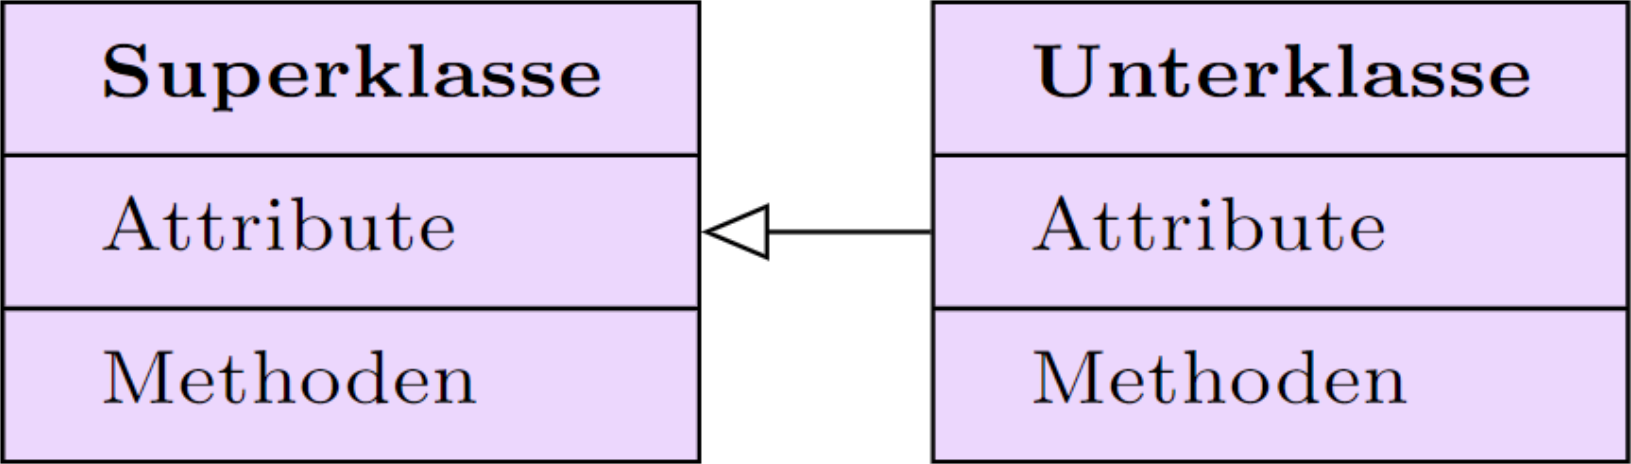
\includegraphics[width=\columnwidth]{pictures/uml.png}    
        }
\end{center}
\end{minipage}
\begin{minipage}{0.4\columnwidth}

Unterklasse erbt (die Attribute und Methoden) von Superklasse. 

\end{minipage}

Dies stellt eine \say{ist ein beziehung} dar. 
Es ist sehr wichtig, dass die Pfeilspitze \colorbox{red!65}{\textbf{genau so!}} aussieht wie in der Darstellung da ansonsten Verwechslungsgefahr mit anderen Mechanismen entstehen könnte.

\subsubsection{UML++}

\noindent
\begin{minipage}{0.6\columnwidth}
\begin{center}
    \ifthenelse{\boolean{tikzumlWorks}}{
        \begin{tikzpicture}

            \umlemptyclass[x=2, y=3]{C1}
    
            \umlemptyclass[x=1, y=1.5]{C2}
            \umlemptyclass[x=3, y=1.5]{C3}
    
            \umlemptyclass{C4}
            \umlemptyclass[x=2]{C5}
            \umlemptyclass[x=4]{C6}
    
            
            \umlinherit{C2}{C1}
            \umlinherit{C3}{C1}
    
            \umlinherit{C4}{C2}
            \umlinherit{C5}{C2}
            \umlinherit{C6}{C3}
    
            \end{tikzpicture}   
        }{
            \includegraphics[width=\columnwidth]{pictures/uml++.png}    
        }
\end{center}
\end{minipage}
\begin{minipage}{0.4\columnwidth}
    Vererbung ist auch über mehrere Stufen Möglich:\\
    Z.b. C4 Erbt alles von C2 und C1
\end{minipage}

\subsubsection{Syntax}

\lstinputlisting{code/vererbung_syntax.cpp}

Die Sichtbarkeit ist durch das Public definiert. 
Es ist möglich die Sichtbarkeit aller Attribute und Methoden einzuschränken. 
Mit \textbf{Public} wird alles mit der originalen Sichtbarkeit übernommen. 
Mit \textbf{protected} wird alles was public war protected. 
Mit \textbf{private} wird alles private (nicht sehr nützlich).

\begin{center}
    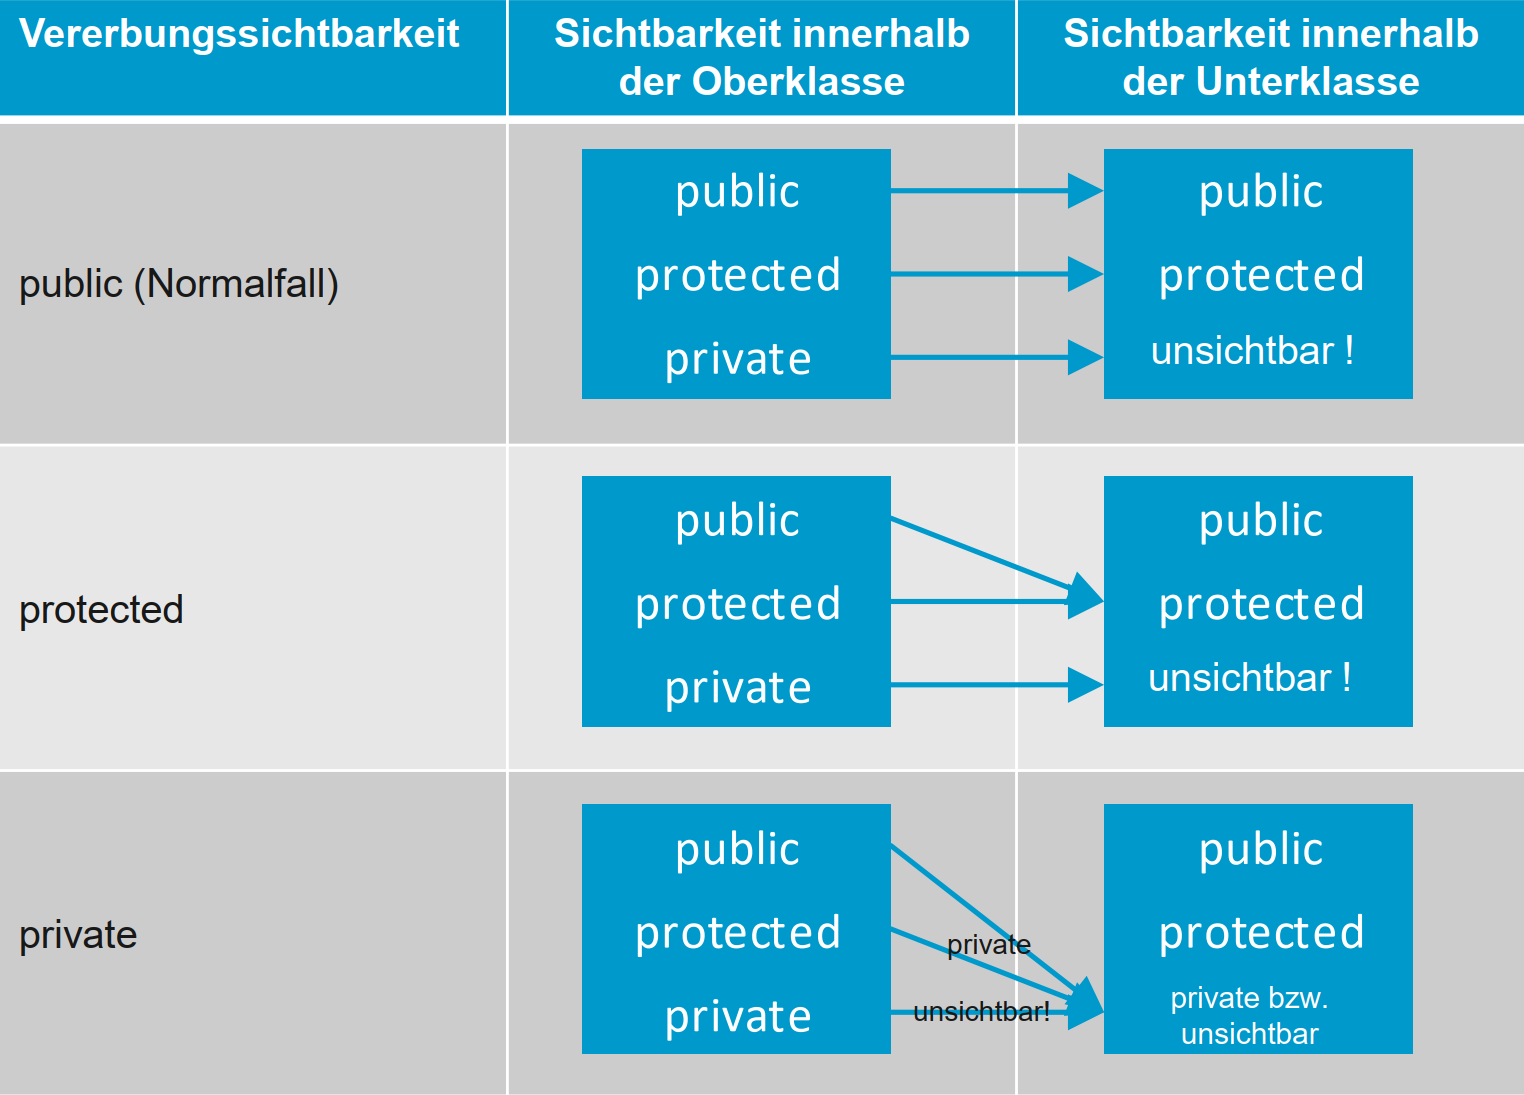
\includegraphics[width=0.7\columnwidth]{pictures/Vererbung.png}    
\end{center}

Wird eine Vererbung private durchgeführt, sind keine Attribute oder Methoden mehr sichtbar.

\subsubsection{Ctor / Dtor chaining}

Grundsätzlich initialisieren ctors nur die eigene Klasse. 
Dh Superklassen initialisieren sich selbst. 
Eine Subklasse initialisiert sich, indem sie zunächst einen Ctor der Superklasse aufruft und danach sich selbst \textbf{IMPLIZIT}. 
Man kann das auch explizit machen:

\lstinputlisting{code/ctor_unterklasse.cpp}

Note: Da der Konstruktor aufgerufen wird kann auch ein evtl Private Attribut der Oberklasse initialisiert werden.
Gleiches gilt mit dem Dtor, nur umgekehrte Reihenfolge (erst wird der Dtor von der subklasse aufgerufen, dann.....).

\subsection{Überschreiben von Methoden}

Geerbte Funktionen können \say{überschrieben} werden. 
Die Unterklasse definiert eine neue Methode mit demselben Namen.
Allerdings kann es dann zu Mehrdeutigkeit kommen:\\
Im folgenden Beispiel haben eine Subklasse und eine Oberklasse eine print Funktion welche \textbf{nicht} virtual gekennzeichnet ist:

\lstinputlisting{code/methodenueberschreiben.cpp}

Dieses Beispiel soll zeigen, dass Pointer, welche eigentlich von einer Oberklasse auf eine Unterklasse zeigen auf die \say{Eigenen} Funktionen der Oberklasse zeigt, solange diese nicht überschrieben worden sind.
Dies kann als Verhalten gewünscht sein. 

\subsection{virtual, scopeoperator, override und final}

\subsubsection{virtual}\label{Virtual}

Mit \textbf{virtual} kann eine Methode gekennzeichnet werden, dass diese Methode von einer Unterklasse überschrieben wird.
Somit würde das obige Beispiel nicht mehr funktionieren und es wird immer die Printfunktion der Unterklasse aufgerufen. 
In einer Unterklasse ist virtual nicht mehr zwingend zu schreiben.
Eine Klasse mit einer virtuellen Funktion wird als Polymorph bezeichnet.

\subsubsection{Virtual beim Dtor}

Ist eine Methode als virtual deklariert, so muss der Dtor \textbf{ZWINGEND} auch als virtual deklariert werden.

\subsubsection{Override}

Soll eine Methode eine geerbte Methode ersetzen so muss diese mit \say{Override} gekennzeichnet werden. 
Solch eine Methode ist automatisch auch virtual.
Der Compiler kann so überprüfen, ob eine virtual Methode vorhanden ist.

\subsubsection{Final}

Final kann zum einen verbieten, dass eine Methode einer Klasse überschrieben wird
(Logischerweise geht das nur bei virtuellen Methoden). 
Zum anderen kann sie auch das weitere Erben einer Klasse verbieten. 

\subsubsection{Scopeoperator}

Per Scopeoperator kann (::) eine Methode aus einer Oberklasse gezielt aufgerufen werden. 
Mit diesem wird garantiert die Funktion welche definiert wird aufgerufen, egal ob diese aufgrund virtual überschrieben wird. 

\lstinputlisting{code/virtual.cpp}

\subsubsection{RTTI / Typing / Binding}

Wird kein Virtual verwendet, nennt man das \textbf{static binding}. 
Mit virtual wird es \textbf{dynamic binding} genannt, da erst bei Laufzeit bekannt ist, um welchen Pointer es sich handelt.\\
Um bei Laufzeit herauszufinden, um welchen Typ es sich handelt kann die \textbf{Run-time Type Information} verwendet werden. 
Dies geschieht mit der \textbf{typeid()} Funktion aus dem Header \textbf{$<$typeinfo$>$}\\
typeid gibt ein std::type\_info zurück. 

\lstinputlisting{code/RTTI.cpp}

\subsubsection{Imlementation von RTTI}

Das RTTI System arbeitet meistens mit einem so genannten V-Table in dem zu allen(evtl geerbten) virtuellen Methoden ein Pointer definiert ist. 
Die Klasse erhält zusätzlich einen V-table Pointer. 
Zur Laufzeit kann die Instanz via V-table die korrekte Methode ermitteln.\\

Das folgende Beispiel zeigt das die Memory-map von einem Array mit 2 Oberklassenpointer. 
Ein Pointer zeigt auf eine Oberklasse, die anderen auf Unterklassen, welche virtuelle Methoden überschrieben haben. 
Der V-pointer der Ober- und Unterklasse ist darum unterschiedlich / sie zeigen nicht auf denselben Vtable. 
Die Unterklassen zeigen wiederum auf denselben Vtable.  

\begin{center}
    \ifthenelse{\boolean{tikzumlWorks}}{
        \includesvg[width = \linewidth, inkscapelatex=false]{svg/vtable.svg}    
    }{
        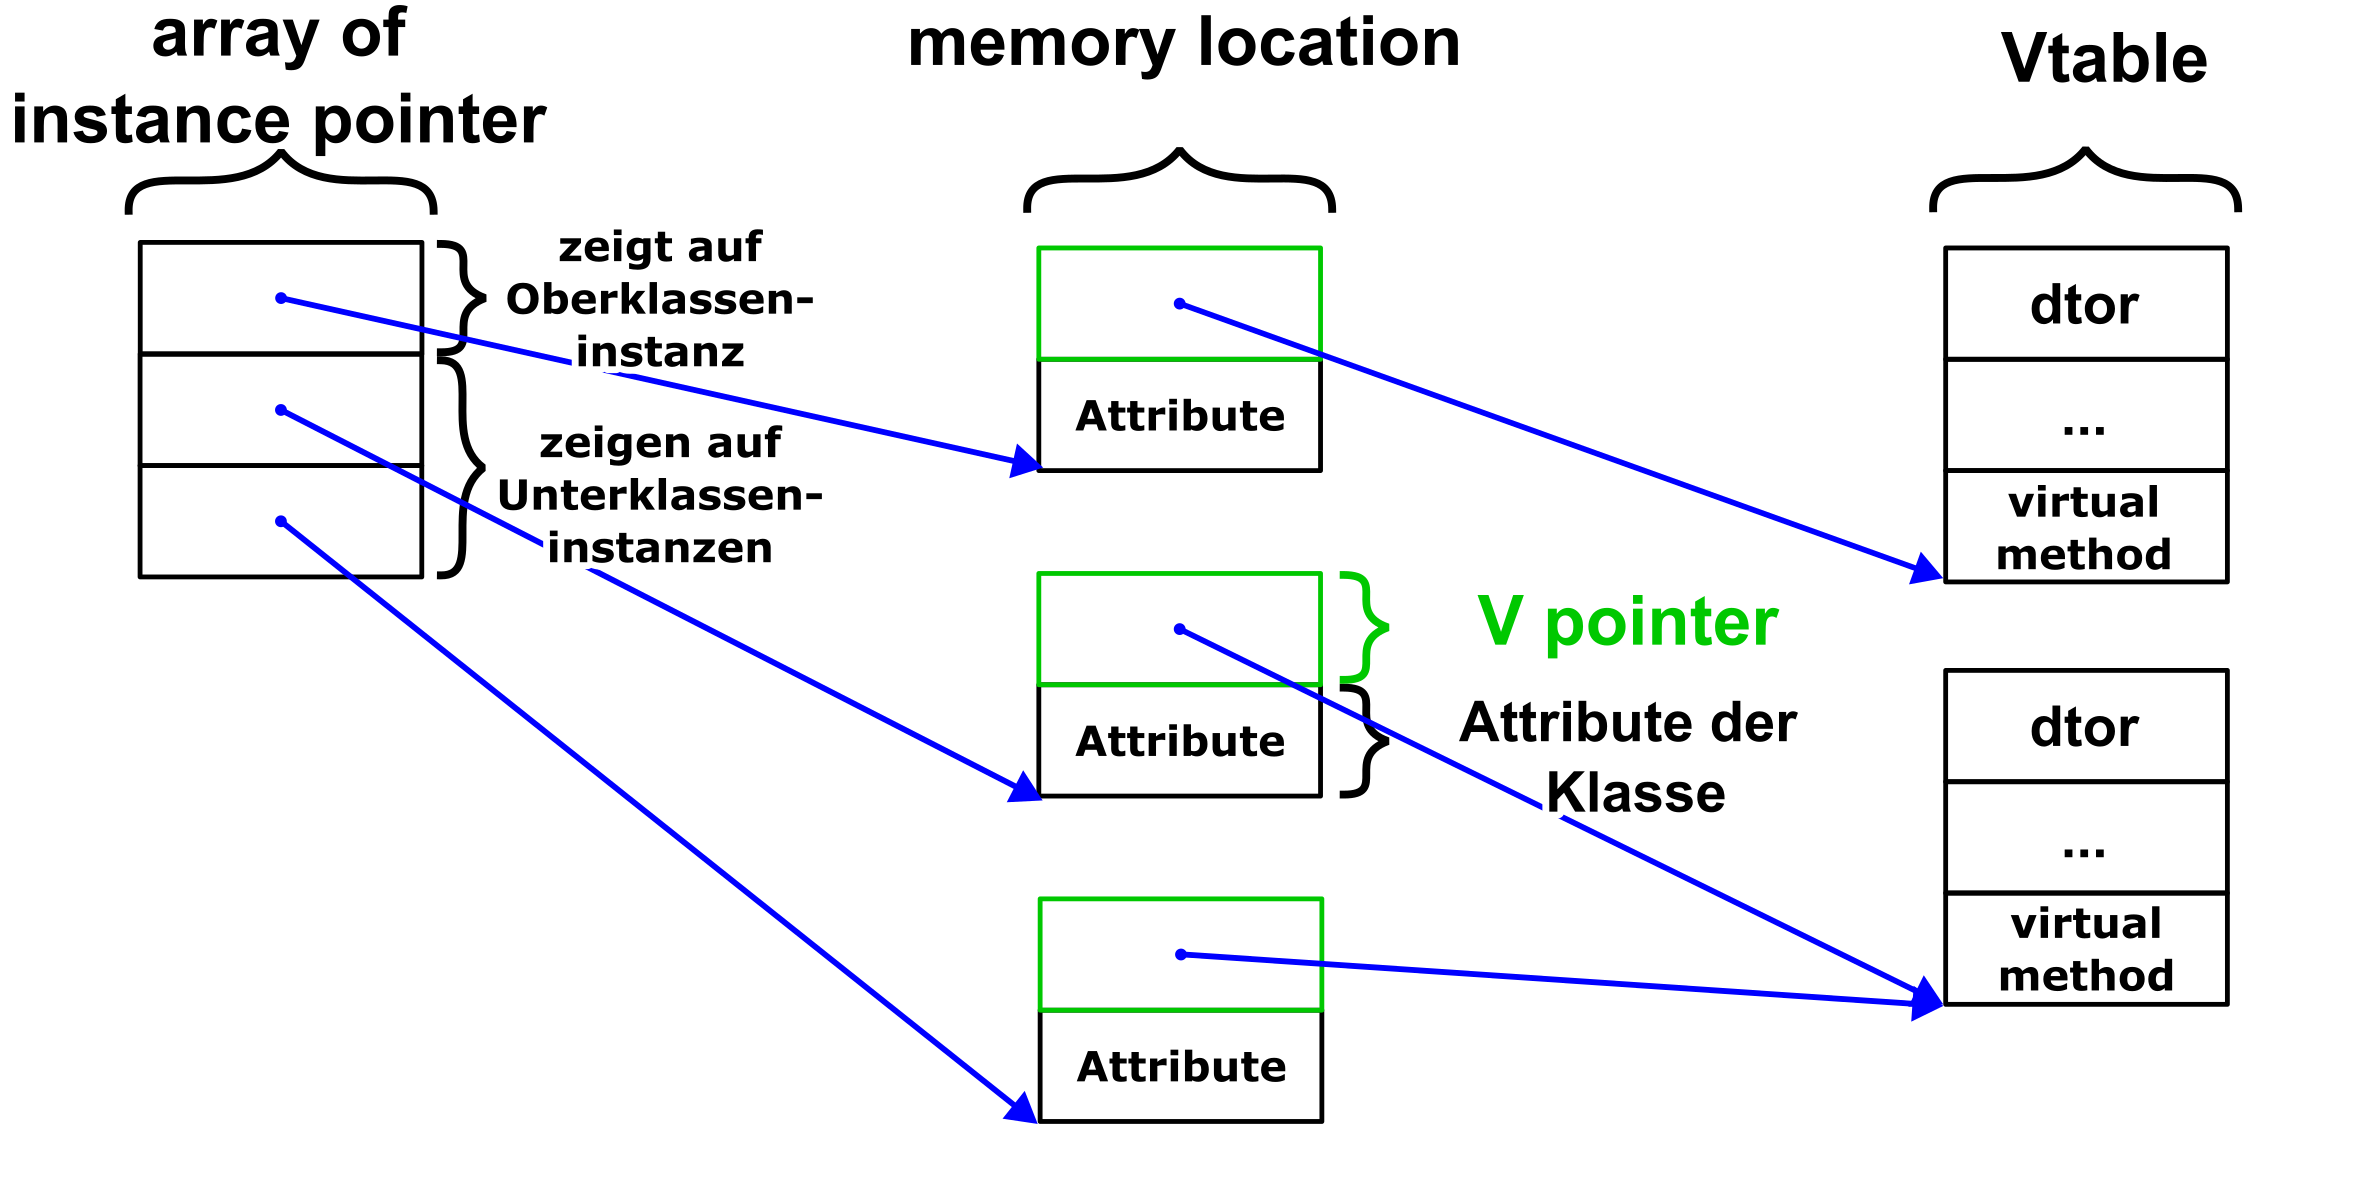
\includegraphics[width=\columnwidth]{pictures/vtable.png}  
    }
\end{center}

\nextcol

\subsection{Abstrakte Klassen}

Wenn Klassen zwar festlegt, dass eine Methode da ist, diese aber noch nicht implementieren, nennt man das eine abstrakte Methode. 
Man spricht dann von einer abstrakten Klasse.
Eine abstrakte Methode wird in UML \textit{\textbf{kursiv}} dargestellt.
Es ist egal, ob die abstrakten Methoden selbst definiert sind oder geerbt. 
Abstrakte Klassen kann man nicht instanziieren.
Es gibt kein spezielles Schlüsselwort dafür, man weist der Methode bei Definition 0 zu: 

\lstinputlisting{code/abstraktemethode.cpp}

\subsection{Organisation der H files}

Generell gilt immer noch: Jedes H File hat ein Cpp File. 
Allerdings können Unterklassen in ein H File zusammengefasst werden, falls diese nicht allzu Umfänglich sind. 
Ansonsten sollte ein neues H File erstellt werden. 
Für abstrakte Klassen fällt die Implementierung in einem Cpp file weg.

\subsection{Mehrfachvererbung}

Folgender Vererbungszweig ist möglich:\\
\noindent
\begin{minipage}{0.5\columnwidth}
    \begin{center}
        \ifthenelse{\boolean{tikzumlWorks}}{
            \begin{tikzpicture}
    
                \umlemptyclass[x=1, y=4]{C1}
        
                \umlemptyclass[x=0, y=2]{C2}
                \umlemptyclass[x=2, y=2]{C3}
        
                \umlemptyclass[x=1]{C4}
                
                \umlinherit{C2}{C1}
                \umlinherit{C3}{C1}
        
                \umlinherit{C4}{C2}
                \umlinherit{C4}{C3}
        
                \end{tikzpicture}   
            }{
                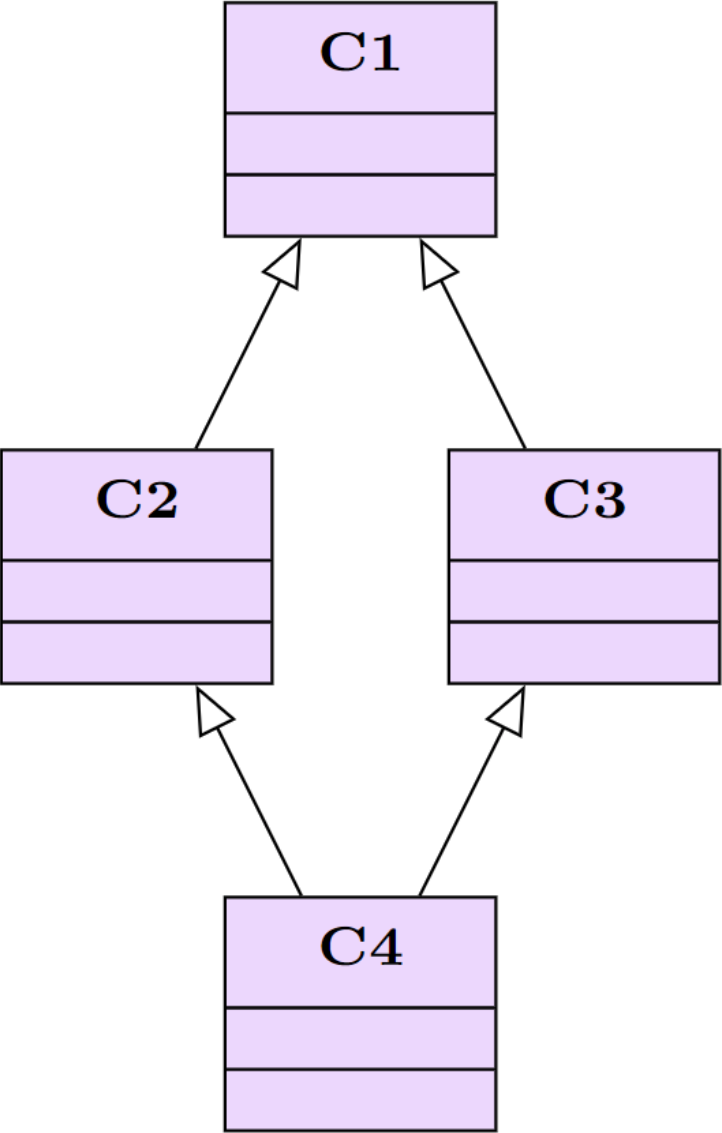
\includegraphics[width=0.7\columnwidth]{pictures/Mehrfachvererbung.png}    
            }
    \end{center}  
\end{minipage}
\begin{minipage}{0.5\columnwidth}
Solche Gebilde sind zwar möglich, sollten jedoch vermieden werden, da schnell sehr kompliziert und kaum lesbar. 
Es entsteht schnell Mehrdeutigkeit durch die verschiedenen Erbzweige.\\
Bei der Definition einer Klasse können weitere Oberklassen mit einem Komma getrennt angegeben werden :

\end{minipage}

\lstinputlisting{code/Mehrfachvererbung.cpp}

\subsection{Static} 

Static im Zusammenhang mit Klassen bindet eine Methode oder ein Attribut an die Objektklasse und nicht an die Objektinstanz (ähnlich zu Python Klassenvariablen).


\subsubsection{Methoden}

Static Methoden müssen im Header-File deklariert und im Cpp-File definiert werden. 
Sie dürfen nur auf Static definierte Attribute zugreifen da keine Objektinstanz vorhanden. 
Hauptanwendungen sind Hilfsfunktionen wie Funktionsaufrufcounter oder Umrechnungsfunktionen. 
Bei der Deklaration wird der Klassennamen verwendet (siehe Bsp). 

\subsubsection{Attribute}

Static Attribute müssen im H deklariert und im Cpp File definiert werden. 
Sie werden verwendet für z.B. Objektspezifische Konstanten oder im Zusammenhang mit Static Counter. 

\subsubsection{Bsp}

\lstinputlisting{code/static.cpp}

        \section{Memorymanagement}

Es gibt verschiedene Gründe warum, nicht immer gleich viel Speicher verwendet wird z.B. da nicht unbegrenzt vorhanden ist.
Speicher wird nur dann verwendet wenn er wirklich gebraucht wird. 
Das Memorymanagement muss aktiv beachtet werden.
Es wird zwischen automatischen und manuellen Speichermanagement unterschieden. 

\subsection{Automatisch}

Automatisches Speichermanagement wird anhand der Lebenszeit einer Variable festgestellt und während dem Programmieren bereits festgelegt. 
Der Speicher liegt auf dem sogenannten \textbf{Stapel / Stack}.\\
Wird eine Funktion aufgerufen werden die benötigten Variablen auf dem Stack definiert. 
Ebenso wird eine Return Adresse zur Funktion, die die Funktion aufgerufen hat abgelegt.
Wie die Daten angeordnet werden, ist Architektur-abhängig.
Wird die Funktion wieder verlassen, werden die Variablen vom Stack wieder entfernt und zur aufrufenden Funktion zurückgesprungen.  

\subsection{Manuell/dynamisch}

Man kann auch manuell Speicher anfordern. 
Zum Beispiel, falls zur Compilezeit nicht bekannt ist wie viel Speicher gebraucht wird.
Dieser Speicher ist auf dem sogenannten \textbf{Haufen / Heap}.\\
Der Heap ist ein Speicherbereich der vom Betriebssystem bereitgestellt und verwaltet wird.\\
Zur Laufzeit wird Speicherdynamisch angefordert. 
Dieser bleibt so lange belegt bis dieser Manuell wieder freigegeben wird.\\
Es kann aber auch sein, falls der Speicher stark fragmentiert ist, das kein Speicher bereitgestellt werden kann. 
Generell ist bei sehr vollem Speicher das Arbeiten erschwert.

\subsubsection{Speicherlecks}

Falls ein Programm unkontrolliert Speicher aufnimmt oder den ihm zur Verfügung gestellte nicht wieder freigibt, spricht man von einem Speicherleck. 
Diese sind zu verhindern da diese zu einer Systemüberlastung führen und Abstürzen führen.

\subsection{Speichermanagement funktionen}

Es gibt einige Funktionen für Speichermanagement. In c und C++ sind diese leicht verschieden. 
Generell geben diese einen Pointer zurück, welcher auf freien Speicher zeigt. 
\textbf{Diese müssen immer auf einen nullpointer geprüft werden da keine garantie vorhanden ist das überhaupt speicher vorhanden ist!}
Generell sollte mit solchen Pointer immer mistrauisch gearbeitet werden und nach ambschluss immer wider freigegeben werden.

\subsubsection{C: malloc( ) calloc( ), free( ) (Funktionen)}

Malloc() gibt einen Voidpointer(pointercasting nicht vergessen) zurück welche auf eine angeforderte Grösse an Bytes Speicher zeigt. 
Der Speicher ist \textbf{nicht} initialisiert
Calloc() macht dasselbe, initialisiert aber den Speicher auf 0.\\
free() gibt den Speicherbereich wieder frei.

\lstinputlisting{code/mem_mngmt_c.c}

Falls kein Speicher allokiert werden kann, wird ein NULL-pointer zurückgegeben.

\subsubsection{C++: new, delete, new[ ], delete[ ] (Operatoren)}

Der New Operator erstellt ein Pointer welcher auf die mitgegebene Grösse zeigt.
new[ ] macht dasselbe, ausser das dieser ein Array zurückgibt.

Delete([ ]) gibt den Speicher wieder frei. 
Dieser kann auch auf den Nullpointer ausgeführt werden. 
Dieser ist \say{Delete} egal.

\lstinputlisting{code/mem_mngmt_cpp.cpp}

\subsection{Speicheraufbau}

Der Speicheraufbau bildlich dargestellt sieht ungefähr so aus:

\begin{center}
    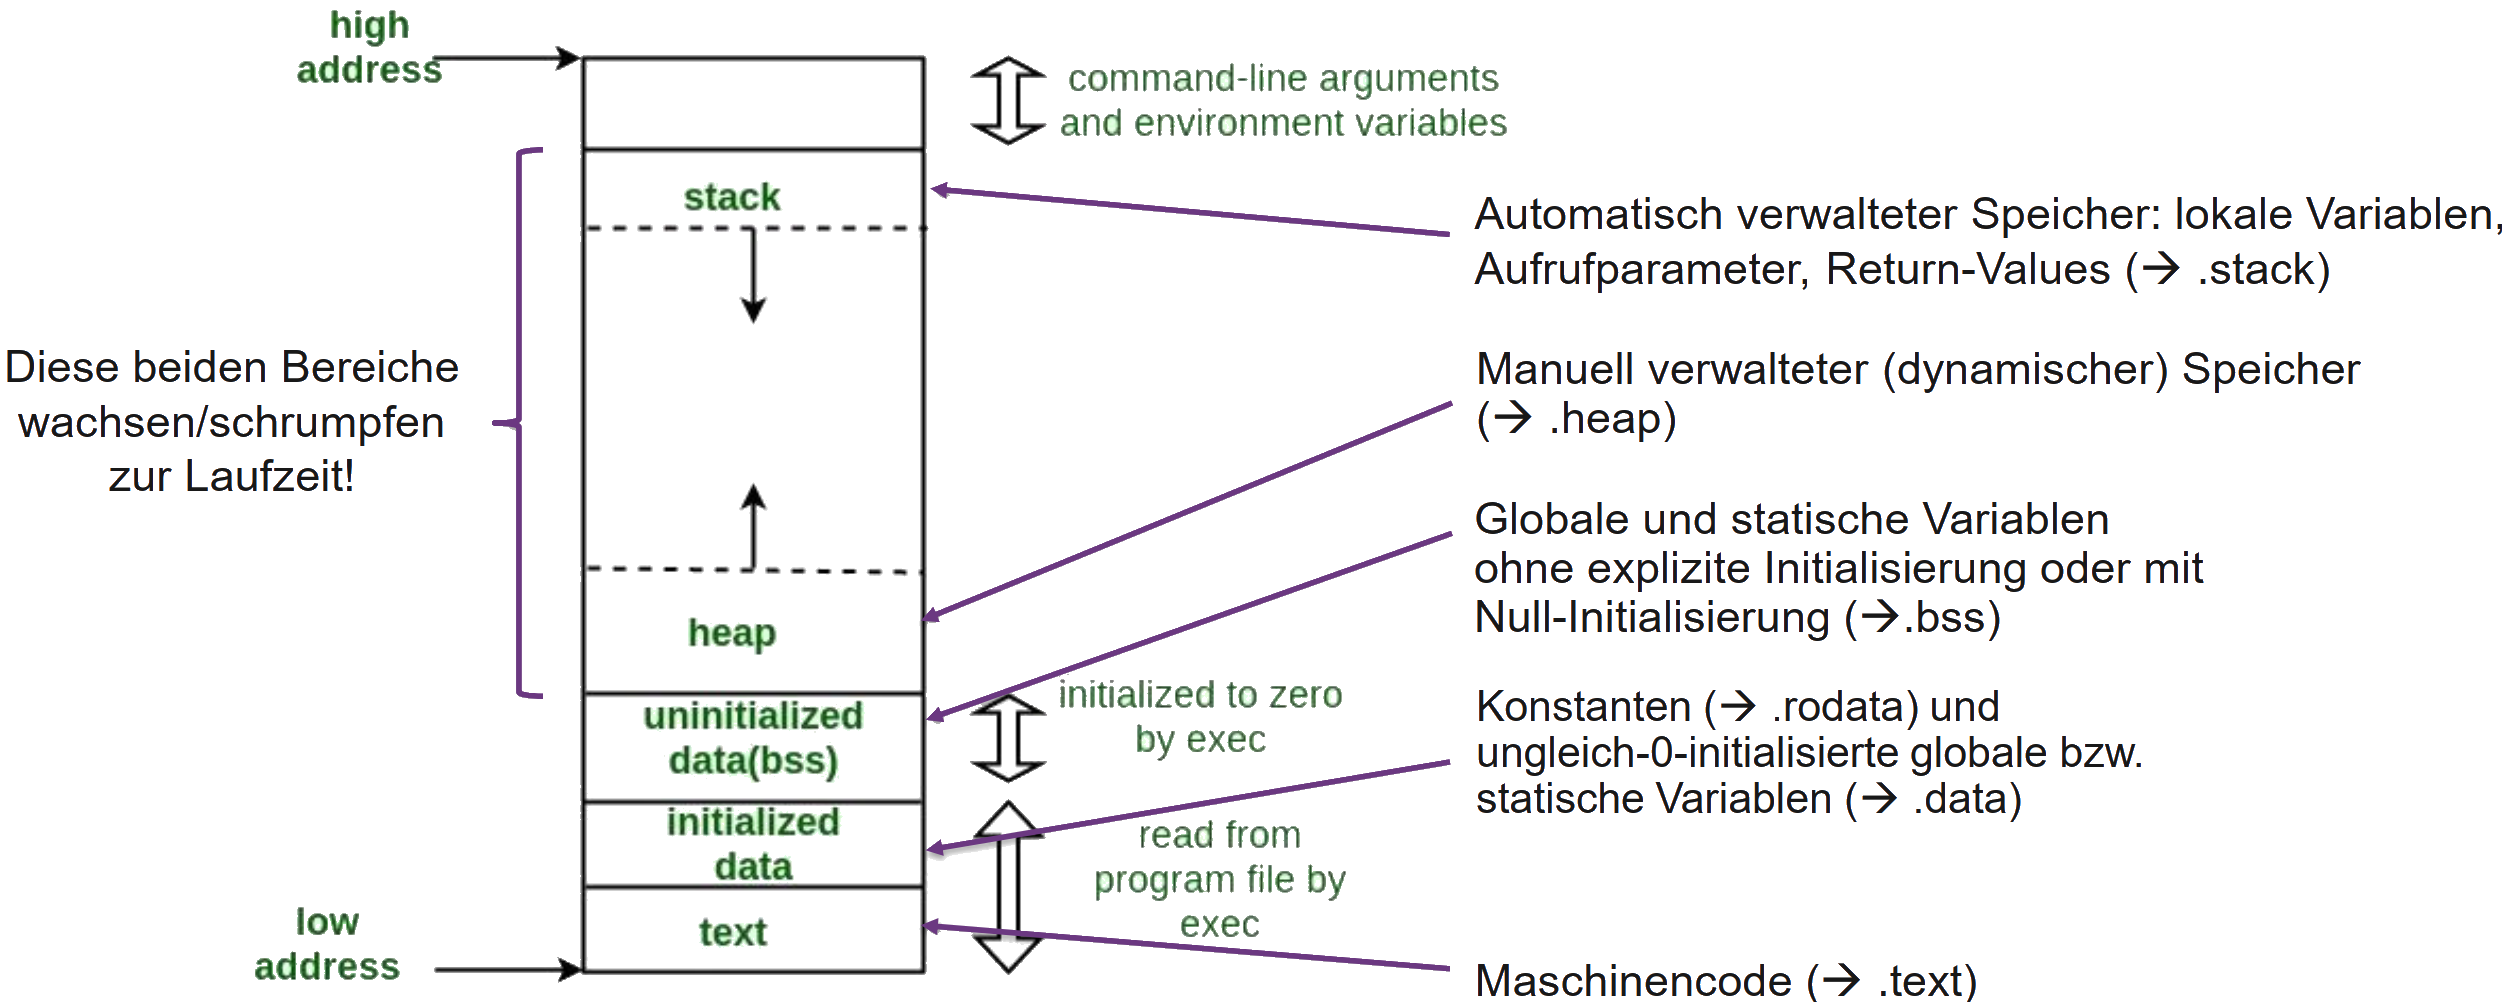
\includegraphics[width=\columnwidth]{pictures/memorylayout.png}  
\end{center}

Je nach Architektur kann es auch sein das die hohen und tiefen Adressen anders herum sind.

\subsection{Referenzen}

Referenzen sind die modernere / eingeschränkte Version von Pointer. 
Wenn möglich sollte immer mit Referenzen gearbeitet werden, dies ist aber nicht immer möglich.\\

Referenzen...
\begin{itemize}[itemsep=1pt, parsep=0pt]
    \item wirken wie ein Alias-Name einer Variablen
    \item werden wie normale Variablen verwendet
    \item sind niemals uninitialisiert
    \item haben niemals den Wert nullptr
    \item brauchen nicht immer speicher(Implementation abhängig)
\end{itemize}

Generell helfen Referenzen weniger Fehler in der Programmierung zu machen und weniger Risiken zu haben. 
Pointer werden allerdings weiter für sehr hardwarenahe Programmierung gebraucht. 
Sizeof() liefert die Grösse des Typs, auf der die Referenz zeigt.\\
Beispiel:

\lstinputlisting{code/referenz.cpp}


\subsection{Speicherplatzbedarf von Objekten}

Eine Unterklasse braucht immer mindestens so viel speicher einer Oberklasse.

\subsubsection{Zuweisungen}

Zuweisungen von Oberklasse zu Unterklasse sind in der regel möglich da alle geerbten Attribute ja vorhanden sind. 
Umgekehrt geht das allerdings nicht, da der Speicher dafür nicht initialisiert ist.

\subsection{Type Casting}

\subsubsection{implizit}

Implizites typecasting erlaubt bei numerischen Typen, einigen Pointertypen und Unklasseninstanz zu Oberklassenpointer. 

\subsubsection{Explizit mit C Operator}

Der C Operator \say{()} kann verwendet werden, sollte man aber nicht da keine Unterscheidung bei der Typprüfung (ob statisch oder zur Laufzeit). 

\subsubsection{Explizit const\_cast$<$const typ$>$()}

Hiermit kann die \say{const-ness} oder \say{volatile-ness} ausgehebelt werden. 


\subsubsection{Explizit static\_cast$<$static typ$>$()}

Kann ober und Unterklassenpointer in beide Richtungen casten. 
Unterdrückt auch alle Warnungen bei impliziten Typumwandlung. 
Es findet keine Typprüfung zur Laufzeit statt. 
\textbf{Meist verwendeter}


\subsubsection{Explizit dynamic\_cast$<$dynamic typ$>$()}

Kann Pointertypen auf polymorphe Klassen casten und prüft mit RTTI ob Typ stimmt. 
Falls nicht, wird ein nullptr zurückgegeben.
Kann nicht polymorphe Unterklassen zu einer Oberklasse casten. 


\subsubsection{reinterpret\_cast$<$reinterpret typ$>$()}

Mappt das zugrundeliegende Bittmuster auf neuen Typ. 
Macht keine Typ-Kompatibilitätsprüfung. 
Reinterpretcast ist Platform Abhängig.

\lstinputlisting{code/casting.cpp}

        \section{Makefiles}

Makefiles sollten generell das umsetzten des Codes in Maschinencode vereinfachen.
Es ist eine \say{Skriptingsprache} welche grob nach dem muster \say{Erzeugnis/target} : \say{Abhängigkeiten/Dependency} folgt. 
Dann folgt indentiert der Befehl, um dieses Erzeugnis zu erzeugen.\\
Wenn ein Erzeugnis keine Datei zurückgibt, muss dieser als \say{.PHONY} markiert werden. 
Das verhindert, dass eine Datei mit demselben Namen das Ausführen verhindert.\\
Am besten sieht man das an einem Beispiel:

\lstinputlisting[language = Make, frame=single]{code/make1}

Der Befehl \say{make all} baut nun das Projekt.\\
Sind die o Dateien noch aktuell werden diese nicht erneut kompiliert. 
Das Projektverzeichnis kann einfach durch \say{make clean} aufgeräumt werden.

\subsection{Platzhalter}

In einem Makefile können auch Platzhalter verwendet werden:

\begin{itemize}[itemsep=1pt, parsep=0pt]
    \item \textbf{\$ @} Dateiname des Targets
    \item \textbf{\$ $<$} Dateiname der ersten Dependency des aktuellen Targets
    \item \textbf{\$ $\wedge$} Dateiname aller Dependencies des aktuellen Targets durch Leerzeichen getrennt
\end{itemize}

Mit diesen Mitteln kann ein Professionelleres Makefile erstellt werden:

\lstinputlisting[language = Make, frame=single]{code/make2}

Diese kann relativ universell verwendet werden, um kleinere Projekte zu übersetzen.

        
        \section{Emotional support meme}
        
        \begin{center}
            
\includegraphics[width=\columnwidth]{pictures/ifcondition.png}  
        \end{center}            

	\end{multicols*}
\end{document}
